
\definecolor{PROGRESS}{cmyk}{0.10, 0.10, 0.0, 0.0, 1.00}
\definecolor{TODO}{cmyk}{0.0, 0.10, 0.10, 0.00, 1.00}
\definecolor{DONE}{cmyk}{0.10, 0.0, 0.10, 0.0, 1.0}


\newcommand{\REVIEW}[3]{
  \begin{tcolorbox}[colback={#1}]
    {\bf {#1}. {#2}}
 \end{tcolorbox}
  \begin{quote}
    {#3}
  \end{quote}
}

REVISION DUE: 01.12.2021




\section{Additional actions taken}


\REVIEW{DONE}{Using the JDS template} {We used the new JDS \LaTeX
  template available from the Journal page instead of the older one
  that we used. This also includes The change of citations in brackets
  when cited. URLs have been added with the standard urlbst tool so
  they can be used in the refernces. The jdsurl.bst is included in the
  source.}



\section*{Reviewer 1}

The revised manuscript is much smoother than the first version, but I
still feel that less than sufficient care was put into the
writing. The reviewer pointed some in the pdf report. I have some
additional editorial suggestions:

\bigskip

  \REVIEW{PROGRESS} {Submit the point-by-point response to the
    reviewer's comments and my comments in a pdf file.}{The original
    submisison web page had a field to enter the comments as text
    which we used. We just added ``see attached PDF'' to make it
    easier for reviewers as suggested by the editor.}

  \REVIEW{DONE} {Needs page number (line number) for ease of
    referencing in the review.}
  {Page numbers and line numbers were
    activated with the review style from the new JDS \LaTeX{}
    template}

  \REVIEW{DONE} {Do not italicize in the text.}
  {All italicized text
    have been removed.  Formulas enclosed in dollar signs are in
    italized text as is default for the JDS document style.}


  \REVIEW{DONE} {AICov needs to be defined in the abstract.}
  {We added ``We present the architecture of an artificial
    intelligence enhanced COVID-19 analysis (in short AICov)''
  in the abstract. We also defined COVID-10 in the abstract.}

\REVIEW{PROGRESS}{Acronyms need to be defined at their first occurrences
  (e.g., AI in the intro). An acronyme table is included in table 1,
  we added the following acronyms to the paper}
  {All acronyms have been defined at their first usage. In addition
    we have added a section Acronyms in which all acronyms are listed
    to make it easier for the reader to look them up in case they are
    used later on in the paper. All riskfactors have been capitalized.
    The duplicated Risk factors were removed.
  }
  

\REVIEW{TODO}{Figure 2: please present the equations as equations. The
  notations used in the equation need a full check (e.g., h is used as
  both the dimension and vector). I'd like to see a clear distinction
  between inputs/outputs and parameters. I'd suggest that the inputs
  be set up before the equations are presented.}
  { todo}


\REVIEW{TODO}{Regenerate the figures into pdf format (the current
  jpg/png figures blur when zoomed in).}
  { todo}


\REVIEW{DONE}{Table 2: consider reformating it; it would not fit the
  page width in print.}
  { Table 2 has been reformatted. It was previously fit in the column
    with resize box. While rotating the headers the font is
    increased. The table still fits in the column as it still uses
    resizebox.}

\REVIEW{DONE}{Table 3: tidy the headers.}
  { The headers have been cleaned up and linebreaks were introduced so
    the resizebox of the table presents the table now larger} 

\REVIEW{TODO}{Figure 5-6: can be combined to one figure with two
  panels (using ggplot2 and save the space of the labels of the
  horizontal axis).  }
  { todo}


\REVIEW{TODO}{Figure 7-8: can be one figure with two panels; pop
  density 2010 needs to be cleaned.}
  { todo}


\REVIEW{PROGRESS}{Figure 9-14: combine into one figure.}
  {

\todo{the lines are missing in the images showing the NONE line}

First we decided to only disaly the top 10 results of each prediction
with a factor. Second we have included the combined picture of it for
deth and cases in the {\bf Figure Combined}. We can include this
figure in the paper if the editor thinks this figure is better or
sufficient. At this tiem we still have included them in a subfigure
(a) and (b) in the paper as the scales on the y axis are
different. Please let us know what you think and we can adapt this.

\begin{figure}[!h]
        \centering
        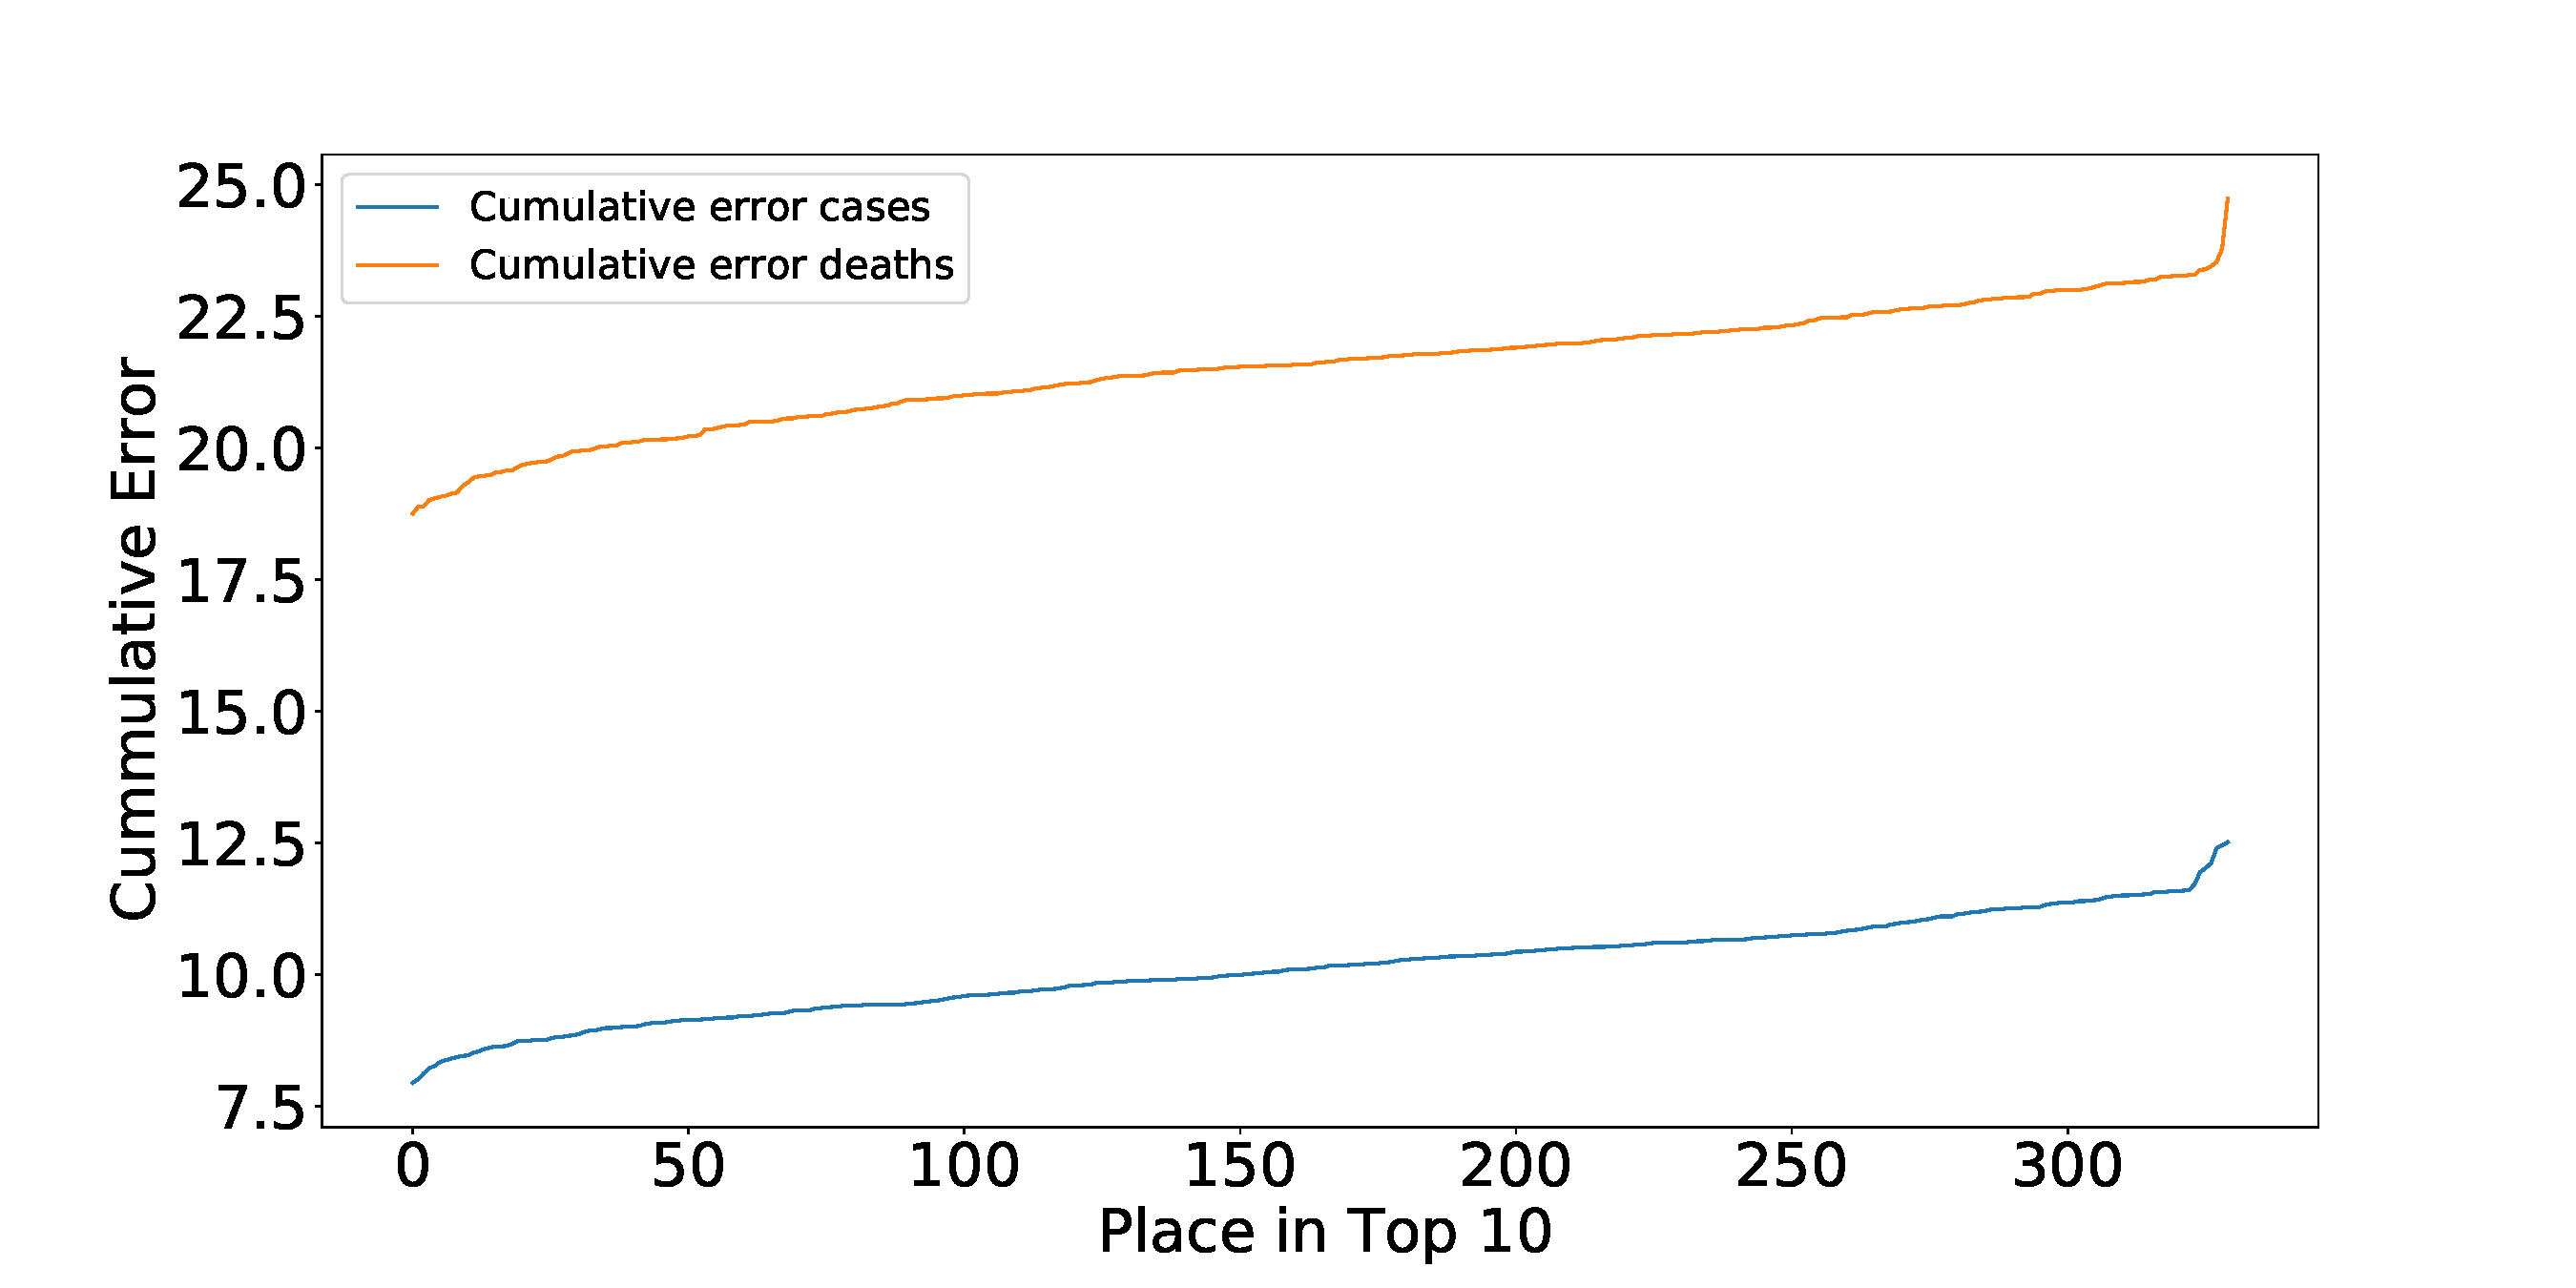
\includegraphics[width=1.0\textwidth]{images/predict/PlaceTop10_CasesAndDeath.pdf}
        
        {\bf Figure Combined} Best predictions for cases over all risk factors.
        
        %\label{fig:place-top10-joint}

\end{figure}

}


\REVIEW{DONE}{Table 4: keep the number of digits consistent.}{
   The digits have been padded with the missing 0 to make them all
    the same length}
  
\REVIEW{TODO}{Reproducibility: submit data/code/README in a
  compressed file as supplementary material, or put them in a public
  repo and give the link under an unnumbered section Supplementary
  Material.}
  { todo}



To submit your revision, please log in to EJMS and submit it as a
revised file to the original submission. Please also include a
detailed description of how you addressed all the points raised by the
reviewers.

\section*{Reviewer 2}

This paper presents AICov, an integrated deep learning framework for
COVID-19 forecasting. It takes into account population covariates, and
uses LSTM and event modeling to do the forecasting. Data integration
is done at a local level. Integration of such information brings
improvement to the prediction accuracy. Despite the authors’ effort to
address my comments in their revision, the paper is still in rough
shape. Please see my comments.

\bigskip

\REVIEW{DONE}{Page 5, please write the full name for REST
  (representational state transfer) when it first appears.}
  { The term has been defined at first usage, we also checked all
    other abbreviations. }



\REVIEW{DONE}{Page 5, line 3 under Requirement 3, “we are developed an
  abstraction API for data” does not read right.
}
  {The sentence has been corrected to: ``To address this requirement, we are developing an
  abstract API for data, analysis, and metadata parameter
  adjustments.''}


\REVIEW{TODO}{Page 6, line 8, what level is “local level”?
}
  {PYNE: todo

  (a) Absract: the term local level has been removed from the abstract and
  replaced by at their ``specific locations''.

  (b) Introduction: The term ``local level'' has been replaced with local which
  according to an editor is suffiecient to refer to data that is
  available for a locality.

  (c) Line \linelabel{comment:level}  ``local level'' has been cahnged as follows
  
We use data on community-specific health and behavioral risk factors
aggregated at the county level from the large-scale longitudinal CDC
Behavioral Risk Factor Surveillance System (BRFSS) surveys
\citep{www-cdc-brfss} and demographic and socioeconomic data from the
\citet{www-sensus}, i.e., both at the county and
census tract, along with the cases and deaths data compiled by
the CDC National Center for Health Statistics (NCHS)
\citep{www-cdc-nchs} and integrate them with other data sources. These
other data sources include

\todo{Pyne}.

}

\REVIEW{PROGRESS}{ Page 7, Table 1, is “CHD” also a percent? If yes
  please modify the description; Percent- blacks and black percent
  both correspond to “Percent of blacks in the population”. Both seem
  to have been used according to Table 3, with difference in the four
  model performance measurements. Do the authors have an explanation
  for this?  }
%
{ (a) The CHD and other values in the table have been updated wether
  they are given in percent.

  (b) There were two different information sources that we originally
  used indicated by the capitalization. However since the submission
  we have improved this data and have now merged all data and
  corrected information for these duplicates, while only presenting
  the one that is more accurate.

  (c) \todo{TODO. fix the values and only have one population value}

}



\REVIEW{DONE}{Page 8, line 5 of Section 5.1, the abbreviation LSTM has
  already appeared before, and the full name can be removed.}
{All acronyms have been defined at first usage. A table has been added
  at the end to make it easier for the reader to look them up.}


\REVIEW{TODO}{What do the two panels in Figure 4 represent? Please give
  clearer description either in the text or figure caption.
}
  { todo}


\REVIEW{DONE}{Section 5.2, paragraph 2 line 6, no need to capitalize for
  the word “Samples”. Line 5 from the bottom, no need to capitalize
  for the word “Insurance”. Please be careful with your writing.
}
{The capitaization has been corrected. The paper has been reviewed by
  2 native English speakers. In addition 2 grammar checking programs
  were used on the entire paper. One of the reviewers serves also as
  editor in other journals.}


\REVIEW{TODO}{Section 5.2, the “order for cases sorted by minimum model
  order” and “order for deaths sorted by minimum model error”
  paragraphs are redundant, as the same information is already
  displayed in the x-legend for Figures 5 and 6.
}
  { todo}


\REVIEW{TODO}{In Table 3, what is the unit for the error terms? The
  errors in Figures 7 and 8 are percentages. If errors in Table 3 are
  also percentages please clearly mark. Also, the numbers in Figures 7
  and 8 do not align with numbers in row 1 of Table 3. Please check
  your numbers with care.
}
  { todo}


\REVIEW{TODO}{Please adjust the location of your figures so they do not
  look pages apart from their interpretations.
}
  { todo}


\REVIEW{TODO}{If I am reading it correctly, Figures 9 and 11 are only
  the “zoom in” versions of partial information from Figure
  13. Similarly for the right column. Why waste space on two more
  figures when you could make Figures 13 and 14 bigger and explain the
  findings?
}
  { todo}


\REVIEW{TODO}{The last paragraph of Section 5.2 suits the
  conclusion/discussion for future work section, not in the middle of
  a paper.
}
  { todo}


\REVIEW{TODO}{Section 5.3, the authors mentioned two way of constructing
  covariates. Since the second way was more complicated while yielding
  no better performance the authors did not use it. Then it can be
  removed without damaging the storyline.
}
  { todo}


\REVIEW{TODO}{The description “We renormalized, so the two basic
  features (following day) contributed 50\% of the loss function” is
  hard to interpret. Please elaborate.
}
  { todo}


\REVIEW{TODO}{Paragraph 2 on page 14, “Selu, Relu and Tanh activations
  gave very similar results while Sigmoid activation was much
  worse. However we still use a Sigmoid function...” is very
  counter-intuitive. Isn’t the point of trying different activation
  functions to better fit the data?  16. Paragraph 3 on page 14, “The
  basic COVID-19 daily data is extensive but compared two approaches
  with and without renormalization, but in this case, we ...” The
  sentence does not read correct. Please check your sentences with
  care!
}
  { todo}


\REVIEW{TODO}{How to interpret the “significant positive correlation” in
  Section 6 from the practical perspective? Also, the term
  “evolution function” made its first appearance in Section 6 without
  any definition or explanation; I suggest either removing the whole
  Section 6, or extend it with clearer definition of evolution
  function.  18. The first two paragraphs do not read like to be in a
  “Conclusion” section. Rather, they better fit into the introduction.
}
  { todo}


\clearpage
